%%%%%%%%%%%%%%%%%%%%%%%%%%%%%%%%%%%%%%%%%%%%%%%%%%%%%%%%%%%%%%%%%%%%%%
% How to use writeLaTeX: 
%
% You edit the source code here on the left, and the preview on the
% right shows you the result within a few seconds.
%
% Bookmark this page and share the URL with your co-authors. They can
% edit at the same time!
%
% You can upload figures, bibliographies, custom classes and
% styles using the files menu.
%
%%%%%%%%%%%%%%%%%%%%%%%%%%%%%%%%%%%%%%%%%%%%%%%%%%%%%%%%%%%%%%%%%%%%%%

\documentclass[12pt]{article}

\usepackage{sbc-template}
\usepackage{graphicx,url}
\usepackage{float}
\usepackage{array}
\usepackage{tabularx}
\usepackage{makecell}

\usepackage{tcolorbox}
\usepackage{minted}

\usepackage[utf8]{inputenc}  

\tcbset{
  codeSnippetStyle/.style={
    colback=gray!10, % cor de fundo mais clara
    colframe=gray!30!, % cor da borda
    title=#1, % título da caixa
    coltitle=black, % cor do título
    boxrule=0.2mm, % espessura da borda
    arc=3mm, % arredondamento dos cantos
    width=\textwidth, % largura da caixa
    boxsep=7pt
  }
}

\newcolumntype{Y}{>{\centering\arraybackslash}X}

\sloppy

%\title{INVESTIGAÇÃO DA ADESÃO DE BOAS PRÁTICAS DE DESENVOLVIMENTO EM PROJETOS OPEN SOURCE FLUTTER: UMA ANÁLISE DE CÓDIGO E MANUTENIBILIDADE}

\title{Análise da Aderência às Boas Práticas de Desenvolvimento em Projetos Open Source Flutter: Primeiros Insights}
\author{Anonymous\inst{1}}

\address{Anonymous \email{\{anonymous\}@anonymous}}

\begin{document} 

\maketitle

\begin{abstract}
This research investigates adherence to best development practices in open-source Flutter projects, focusing on code quality and maintainability. We analyzed 45 projects using SonarQube to identify Best Practice Violations (BPVs). A total of 10,120 BPVs were found, distributed across three severities: 5,149 Minor, 4,273 Major, and 698 Critical. We calculated the Pearson correlation coefficient to confirm the relationship between BPVs and non-commenting lines of code (NCLOC) and between BPVs and cyclomatic complexity. We observed a strong correlation (0.8978) between BPVs and NCLOC, and a moderate correlation (0.4509) between BPVs and complexity. These findings highlight areas for Flutter developers to improve code quality.
\end{abstract}
     
\begin{resumo} 
Esta pesquisa investiga a adesão às melhores práticas de desenvolvimento em projetos open-source Flutter, focando na qualidade e manutenibilidade do código. Analisamos 45 projetos utilizando SonarQube para identificar Violações de Boas Práticas (VBPs). Foram encontradas 10.120 VBPs, distribuídas em três severidades: 5.149 Leves, 4.273 Graves e 698 Críticas. Calculamos o coeficiente de correlação de Pearson para confirmar a relação entre VBPs e linhas de código (LCNC) e entre VBPs e complexidade ciclomática. Observamos uma correlação forte (0.8978) entre VBPs e LCNC, e uma correlação moderada (0.4509) entre VBPs e complexidade. Esses achados destacam áreas para os desenvolvedores Flutter melhorarem a qualidade do código.
\end{resumo}

\section{Introdução}
A evolução tecnológica acelerada tem modificado substancialmente nossa interação com o mundo digital, com os dispositivos móveis emergindo como agentes principais dessa transformação. No Brasil, a média de 1,2 smartphones por habitante causa uma demanda crescente por serviços digitais e aplicativos móveis. Em 2022, por exemplo, os investimentos em tecnologia da informação (TI) corresponderam a 9\% do faturamento das empresas, refletindo também em um aumento significativo no desenvolvimento de aplicativos móveis \cite{FGVcia2023}.

Lançado pelo Google em 2017, o Flutter é um \textit{framework} de código aberto que se tornou popular por permitir que desenvolvedores criem aplicativos que funcionam em múltiplos sistemas operacionais, como Android e iOS, com mínimas alterações no código-fonte, tornando-se uma escolha popular para desenvolvimento multiplataforma \cite{flutter}. Utilizando a linguagem de programação Dart, também desenvolvida pelo Google, o Flutter facilita a escrita de código de alta qualidade e a manutenção a longo prazo. Além disso, se destaca pelo motor gráfico próprio, que oferece consistência e desempenho em diferentes plataformas, e pelo rico ecossistema de pacotes e plugins disponível no Pub, o gerenciador de pacotes do Dart.

Para garantir que os aplicativos desenvolvidos com Flutter mantenham sua robustez e sejam facilmente mantidos ao longo do tempo, é essencial adotar as melhores práticas de desenvolvimento. No contexto do Flutter, isso inclui seguir recomendações da equipe principal do Dart, como a legibilidade, consistência, concisão e eficiência do código \cite{dartBestPractices}. Princípios de código limpo, como clareza, simplicidade e eficiência, além de técnicas de refatoração contínua \cite{fowler1999refactoring}, são fundamentais para assegurar a qualidade técnica do software e facilitar sua manutenção contínua.

Este estudo investiga a adesão às melhores práticas de programação recomendadas pelo time principal do Dart em projetos open source desenvolvidos com Flutter. Este estudo visa responder as seguintes questões de pesquisa:
\begin{enumerate}
\item Qual a prevalência de violações das melhores práticas recomendadas?
\item Com que frequência essas práticas são violadas?
\item Quais tipos de práticas são mais frequentemente violadas?
\end{enumerate}

\section{Metodologia}

Esta seção detalha o procedimento utilizado para avaliar a incidência e o impacto de violações de boas práticas (VBPs) em projetos open source desenvolvidos com Flutter. A metodologia é estruturada em quatro etapas principais: seleção de projetos, configuração das ferramentas de análise, coleta de dados e avaliação dos resultados.

\subsection{Seleção de Projetos}
A seleção apropriada dos projetos é crucial para garantir a relevância da pesquisa. Foram escolhidos projetos open source Flutter hospedados no GitHub, considerando critérios que indicam que o projeto é relevante e atual. Os critérios incluem:
\begin{enumerate}
    \item No mínimo 30 commits, garantindo múltiplas atualizações.
    \item Último commit feito nos últimos 3 anos, assegurando atividade recente.
    \item Mínimo de 30 estrelas no GitHub, indicando relevância na comunidade.
\end{enumerate}

\subsection{Configuração das Ferramentas de Análise}
Utilizamos o SonarQube, uma plataforma reconhecida por sua capacidade de análise de código, para identificar VBPs. O SonarQube foi instalado em um container Docker para garantir um ambiente de análise controlado e consistente. Também configuramos o SonarScanner para coletar dados detalhados dos projetos.

\subsection{Execução da Análise}
A análise foi realizada utilizando o SonarScanner, configurado com um arquivo \texttt{sonar-project.properties} específico para cada projeto. Foram coletadas métricas como número de VBPs, severidade e complexidade ciclomática. A tabela abaixo resume os passos principais:
\begin{enumerate}
    \item Configuração do ambiente Docker e instalação do SonarQube.
    \item Baixando e instalando o plugin para análise de Dart e Flutter.
    \item Configuração e execução do SonarScanner nos projetos selecionados.
\end{enumerate}

\subsection{Coleta e Armazenamento de Dados}
Os dados foram coletados através da API do SonarQube e armazenados em formato JSON. Utilizamos scripts em Python para automatizar a coleta, tratamento e análise dos dados, garantindo consistência e precisão nos resultados.

\subsection{Análise dos Resultados}
Os resultados foram analisados para identificar a prevalência e severidade das VBPs. Calculamos o coeficiente de correlação de Pearson para avaliar a relação entre VBPs e Linhas de Código Não Comentadas (LCNC) e entre VBPs e complexidade ciclomática. Os dados foram visualizados por gráficos e tabelas para facilitar a interpretação.

\section{Resultados}

Esta seção apresenta os resultados obtidos a partir da análise dos projetos open source desenvolvidos com Flutter, com foco na avaliação da adesão às melhores práticas de desenvolvimento.

\subsection{Análise de Violações de Boas Práticas (VBPs)}
Foram analisados 45 projetos utilizando o SonarQube para identificar VBPs. No total, foram encontradas 10.120 VBPs, distribuídas em três níveis de severidade.

\begin{figure}[H]
\centering
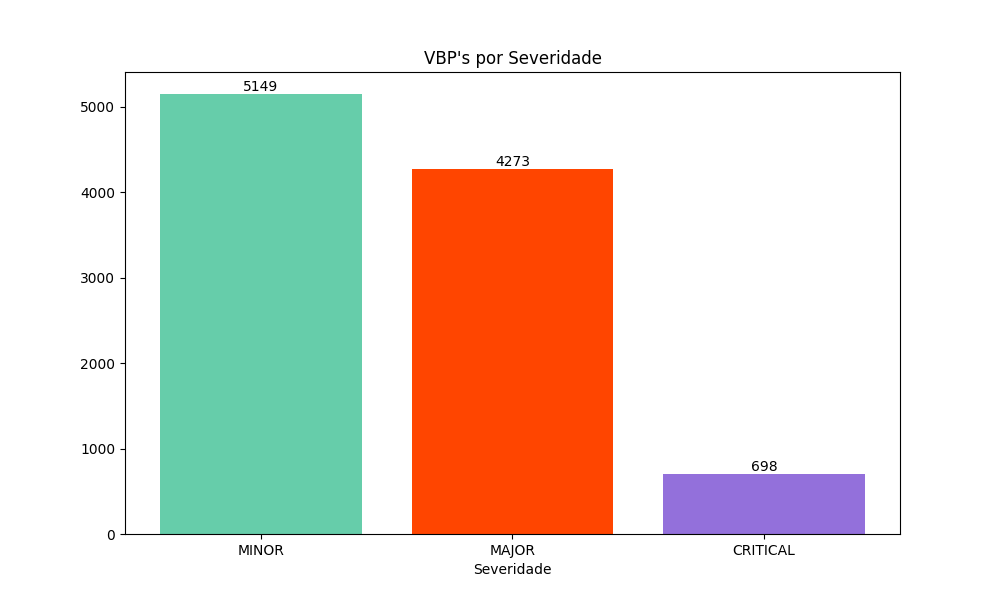
\includegraphics[width=.85\textwidth]{severity_distribution.png}
\caption{Distribuição das VBPs por Severidade}
\label{fig:vbps_severity_distribution}
\end{figure}

\subsection{Correlação entre VBPs e Linhas de Código Não Comentadas (LCNC)}
Calculamos o coeficiente de correlação de Pearson para avaliar a relação entre VBPs e o número de LCNC. Observamos uma correlação forte (\textit{r} = 0.8978), indicando que mais linhas de código estão associadas a mais VBPs.

\begin{figure}[H]
\centering
\includegraphics[width=.85\textwidth]{vbps_vs_lcnc.png}
\caption{Correlação entre VBPs e LCNC}
\label{fig:vbps_vs_lcnc}
\end{figure}

\subsection{Correlação entre VBPs e Complexidade Ciclomática}
Também analisamos a correlação entre VBPs e complexidade ciclomática, resultando em uma correlação moderada (\textit{r} = 0.4509). Isso sugere que projetos com maior complexidade ciclomática tendem a ter mais VBPs.
\begin{figure}[H]
\centering
\includegraphics[width=.85\textwidth]{vbps_vs_complexidade.png}
\caption{Correlação entre VBPs e Complexidade}
\label{fig:vbps_vs_complexidade}
\end{figure}

\subsection{Regras Mais Violadas}
A Figura~\ref{fig:rule_distribution} mostra a distribuição das regras de boas práticas mais frequentemente violadas nos projetos analisados. As siglas das regras são usadas para facilitar a visualização.

\begin{figure}[H]
\centering
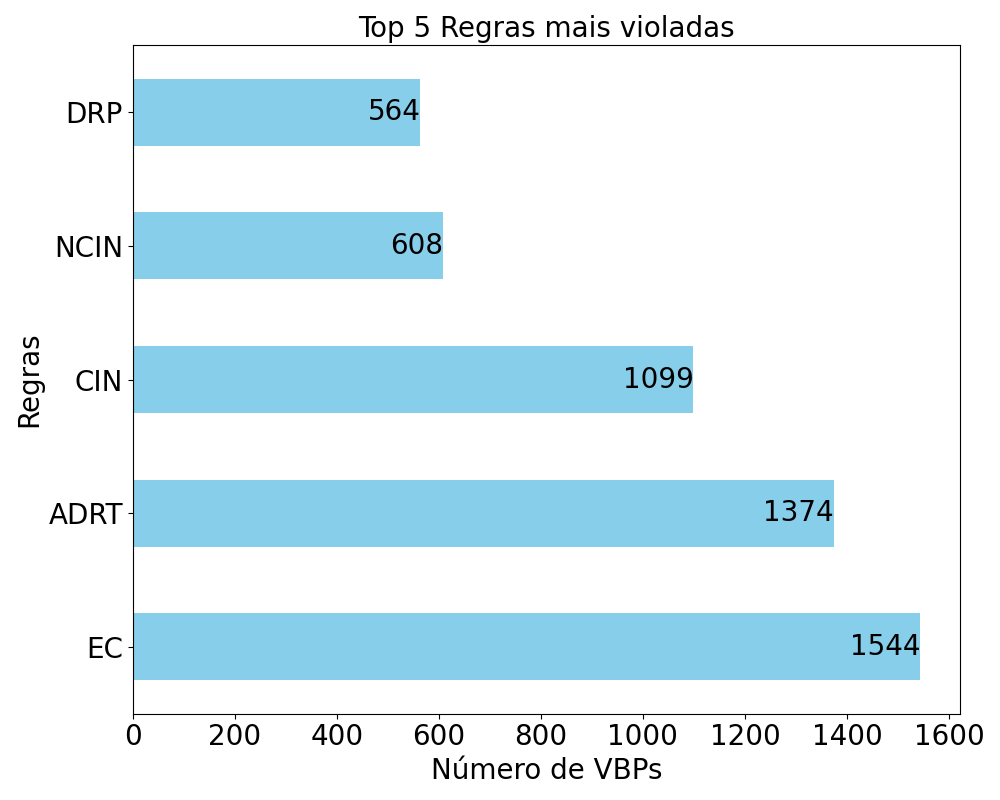
\includegraphics[width=.75\textwidth]{rule_distribution.png}
\caption{Distribuição das Regras Mais Violadas}
\label{fig:rule_distribution}
\end{figure}

% A Tabela~\ref{tab:vbps_description} apresenta a descrição das siglas usadas no gráfico acima, detalhando cada uma das violações de boas práticas identificadas.

% \setlength{\extrarowheight}{3pt}
% \begin{table}[H]
% \centering
% \caption{Descrição dos VBPs Mais Frequentes}
% \label{tab:vbps_description}
% \begin{tabularx}{\textwidth}{|>{\centering\arraybackslash}p{1.5cm}|X|}
% \hline
% \textbf{Sigla} & \textbf{Descrição} \\ \hline
% EC & \makecell[l]{\textbf{Exhaustive Cases:} Verifica se todas as possibilidades em uma enumeração\\ são cobertas.} \\ \hline
% ADRT & \makecell[l]{\textbf{Always Declare Return Types:} Garante que todas as funções tenham tipos\\ de retorno declarados.} \\ \hline
% CIN & \makecell[l]{\textbf{Constant Identifier Names:} Verifica se os nomes das constantes estão em\\ conformidade com as convenções de nomenclatura.} \\ \hline
% NCIN & \makecell[l]{\textbf{Non Constant Identifier Names:} Verifica se os nomes dos identificadores\\ não constantes estão em conformidade com\\ as convenções de nomenclatura.} \\ \hline
% DRP & \makecell[l]{\textbf{Depend on Referenced Packages:} Garante que as dependências declaradas\\ estejam sendo utilizadas.} \\ \hline
% PVTN & \makecell[l]{\textbf{Prefer Void to Null:} Recomenda o uso de void em vez de null quando\\ apropriado.} \\ \hline
% LPTPA & \makecell[l]{\textbf{Library Private Types in Public API:} Verifica se tipos privados de\\ biblioteca não são expostos na API pública.} \\ \hline
% NLULI & \makecell[l]{\textbf{No Leading Underscores for Local Identifiers:} Evita o uso de sublinha-\\dos à frente de identificadores locais.} \\ \hline
% AFLFC & \makecell[l]{\textbf{Avoid Function Literals in Foreach Calls:} Recomenda evitar literais de\\ função em chamadas de foreach.} \\ \hline
% \end{tabularx}
% \end{table}

\subsubsection{Avoid Function Literals in Foreach Calls (AFLFC)}
Recomenda evitar literais de função em chamadas de \texttt{foreach}. No exemplo abaixo, uma literal de função é passada para o \texttt{forEach}.

\begin{tcolorbox}[codeSnippetStyle={Grocery-App/lib/presentation/my\_bag\_page/controller/my\_bag\_controller.dart}]
\begin{minted}[breaklines, fontsize=\footnotesize]{dart}
onSelected(dynamic value) { 
  selectedDropDownValue = value as SelectionPopupModel; 
  myBagModelObj.value.dropdownItemList.forEach((element) {
    element.isSelected = false; 
    if (element.id == value.id) {
      element.isSelected = true;
    }
  });
  myBagModelObj.value.dropdownItemList.refresh(); 
}
\end{minted}
\end{tcolorbox}

\subsubsection{No Leading Underscores for Local Identifiers (NLULI)}
É sugerido evitar o uso de sublinhados à frente de identificadores locais. No exemplo abaixo, o identificador \texttt{\_currentSong} usa um sublinhado no início.

\begin{tcolorbox}[codeSnippetStyle={flutter-tunein/lib/services/musicService.dart}]
\begin{minted}[breaklines, fontsize=\footnotesize]{dart}
final Tune? _currentSong = _playerState$.value.value;
\end{minted}
\end{tcolorbox}

\subsubsection{Library Private Types in Public API (LPTPA)}
Verifica se tipos privados de biblioteca não são expostos na API pública. No exemplo abaixo, o tipo privado \texttt{\_QuickCalculationQuestionViewState} é usado em uma API pública.

\begin{tcolorbox}[codeSnippetStyle={math-metrix/lib/src/ui/quickCalculation/quick\_calculation\_question\_view.dart}]
\begin{minted}[breaklines, fontsize=\footnotesize]{dart}
_QuickCalculationQuestionViewState createState() => _QuickCalculationQuestionViewState();
\end{minted}
\end{tcolorbox}

\subsubsection{Prefer Void to Null (PVTN)}
Recomenda o uso de \texttt{void} em vez de \texttt{null} quando apropriado. No exemplo abaixo, o tipo \texttt{Null} é usado, mas deveria ser substituído por \texttt{void}.

\begin{tcolorbox}[codeSnippetStyle={admin-portal/lib/ui/auth/login\_view.dart}]
\begin{minted}[breaklines, fontsize=\footnotesize]{dart}
final Completer<Null> completer = Completer<Null>();
\end{minted}
\end{tcolorbox}


\subsubsection{Depend on Referenced Packages (DRP)}
Garante que as dependências declaradas estejam sendo utilizadas. No exemplo abaixo, o pacote \texttt{collection} é importado, mas não é referenciado no código.

\begin{tcolorbox}[codeSnippetStyle={openreads/lib/ui/statistics\_screen/widgets/read\_stats\_by\_month.dart}]
\begin{minted}[breaklines, fontsize=\footnotesize]{dart}
import 'package:collection/collection.dart';
\end{minted}
\end{tcolorbox}


\subsubsection{Non Constant Identifier Names (NCIN)}
Verifica se os nomes dos identificadores não constantes estão conforme as convenções de nomenclatura. No exemplo abaixo, o identificador \texttt{SettingService} não segue a convenção de nomenclatura recomendada para identificadores não constantes.

\begin{tcolorbox}[codeSnippetStyle={flutter-tunein/lib/pages/library/tracks.page.dart}]
\begin{minted}[breaklines, fontsize=\footnotesize]{dart}
final SettingService = locator<settingService>();
\end{minted}
\end{tcolorbox}


\subsubsection{Constant Identifier Names (CIN)}
Verifica se os nomes das constantes estão conforme as convenções de nomenclatura. No exemplo abaixo, a constante \texttt{TITLE\_ABOUT} não segue a convenção de nomenclatura recomendada para identificadores constantes.

\begin{tcolorbox}[codeSnippetStyle={WhatTodo/lib/utils/keys.dart}]
\begin{minted}[breaklines, fontsize=\footnotesize]{dart}
static const TITLE_ABOUT = "titleAbout";
\end{minted}
\end{tcolorbox}

\subsubsection{Always Declare Return Types (ADRT)}
É recomendado que todos os métodos tenham tipos de retorno explicitamente declarados. No exemplo abaixo, o método \texttt{getUserType} não possui um tipo de retorno declarado, o que pode levar a problemas de manutenção e compreensão do código.

\begin{tcolorbox}[codeSnippetStyle={gsy\_github\_app\_flutter/lib/page/my\_page.dart}]
\begin{minted}[breaklines, fontsize=\footnotesize]{dart}
getUserType() {
  if (_getStore()?.state.userInfo == null) {
    return null;
  }
  return _getStore()?.state.userInfo?.type;
}
\end{minted}
\end{tcolorbox}

\subsubsection{Exhaustive Case (EC)}
É sugerido que todas as possibilidades em uma enumeração estejam cobertas. No exemplo abaixo, o enum \texttt{EntityType} possui mais opções do que as tratadas no \texttt{switch}, fazendo com que nem todos os casos de uso sejam contemplados, além disso, não há uma opção \texttt{default}.

\begin{tcolorbox}[codeSnippetStyle={gsy\_github\_app\_flutter/lib/page/my\_page.dart}]
\begin{minted}[breaklines, fontsize=\footnotesize]{dart}
String? getDesignId(EntityType entityType) {
    switch (entityType) {
    
      case EntityType.invoice:
        return defaultInvoiceDesignId;
      case EntityType.quote:
        return defaultQuoteDesignId;
      case EntityType.credit:
        return defaultCreditDesignId;
      case EntityType.purchaseOrder:
        return defaultPurchaseOrderDesignId;
    }
    print('## Error: unhandled entity type: $entityType for design id');
    return '';
}
\end{minted}
\end{tcolorbox}

\section{Discussão}
Os resultados obtidos nesta pesquisa fornecem uma visão abrangente sobre a adesão às melhores práticas de desenvolvimento em projetos open-source Flutter. A análise revelou uma correlação forte entre o número de VBPs e o número de linhas de código não comentadas (LCNC), indicando que projetos maiores tendem a apresentar mais violações. Além disso, uma correlação moderada foi observada entre VBPs e a complexidade ciclomática, sugerindo que a complexidade do código também desempenha um papel significativo na qualidade do software.

Comparando com estudos anteriores, nossos achados são consistentes com a literatura que destaca a importância de práticas de codificação estruturada para a manutenibilidade do software. Por exemplo, a duplicação de código, frequentemente apontada como um fator negativo na literatura, também foi identificada como uma área problemática em nossos dados \cite{hunt1999pragmatic}.

Os gráficos das regras mais violadas sugerem áreas específicas onde os desenvolvedores podem concentrar esforços para melhorar a qualidade do código. Regras como `Exhaustive Cases` e `Always Declare Return Types` foram violadas frequentemente, indicando a necessidade de maior atenção a essas práticas.

Para prevenir essas violações e melhorar a qualidade do código, recomendamos fortemente o uso de ferramentas de lint e análise de código durante o desenvolvimento. Ferramentas como o SonarQube, Dart Analyzer e outros linters podem identificar potenciais violações de boas práticas em tempo real, permitindo que os desenvolvedores corrijam problemas antes que eles se tornem significativos. A integração dessas ferramentas no processo de desenvolvimento contínuo pode ajudar a manter um alto padrão de qualidade de código, reduzir a complexidade ciclomática e evitar a duplicação de código \cite{martin2011clean}.

\section{Conclusão}
Esta pesquisa investigou a adesão às melhores práticas de desenvolvimento em projetos open-source Flutter, analisando 45 projetos para identificar Violações de Boas Práticas (VBPs). Foram encontradas mais de 10.000 violações, com uma distribuição significativa entre diferentes severidades.

Os principais achados incluem:
\begin{itemize}
    \item Uma correlação forte entre VBPs e LCNC, indicando que projetos maiores tendem a ter mais violações.
    \item Uma correlação moderada entre VBPs e complexidade ciclomática, sugerindo a importância de manter a complexidade do código sob controle.
    \item Identificação das regras mais frequentemente violadas, fornecendo áreas focais para melhorias na qualidade do código.
\end{itemize}

Esses resultados têm implicações práticas para desenvolvedores de Flutter, destacando áreas específicas onde melhorias podem ser feitas para aderir melhor às práticas recomendadas e melhorar a qualidade e manutenibilidade do código.

Para trabalhos futuros, recomendamos uma análise mais detalhada das causas das violações de boas práticas e a investigação de técnicas automatizadas para auxiliar os desenvolvedores a aderirem a essas práticas. Além disso, seria benéfico expandir o conjunto de dados para incluir mais projetos e explorar a eficácia de diferentes ferramentas e metodologias de análise de código.

\bibliographystyle{sbc}
\bibliography{sbc-template}

\end{document}
